\documentclass[
]{thesis-ekf}
\usepackage[T1]{fontenc}
\PassOptionsToPackage{defaults=hu-min}{magyar.ldf}
\usepackage[magyar]{babel}
\usepackage{mathtools,amssymb,amsthm,pdfpages}
\usepackage{graphicx, url}
\usepackage{placeins}
\usepackage{float}
\usepackage{listings,xcolor,caption,upquote}
\footnotestyle{rule=fourth}

\newtheorem{tetel}{Tétel}[chapter]
\theoremstyle{definition}
\newtheorem{definicio}[tetel]{Definíció}
\theoremstyle{remark}
\newtheorem{megjegyzes}[tetel]{Megjegyzés}

\lstset{
	inputencoding=utf8/latin2,
	basicstyle=\footnotesize\ttfamily,
	columns=fullflexible,
	numbers=left,
	breaklines,
	postbreak=\hbox{$\mathcolor{red}{\hookrightarrow}$\ },
	xleftmargin=2cm,
	xrightmargin=2cm,
	frame=single,
	literate={á}{\'{a}}1
	{é}{\'{e}}1
	{í}{\'{i}}1
	{ó}{\'{o}}1
	{ö}{\"{o}}1
	{ő}{\H{o}}1
	{ú}{\'{u}}1
	{ü}{\"{u}}1
	{ű}{\H{u}}1
	{Á}{\'{A}}1
	{É}{\'{E}}1
	{Í}{\'{I}}1
	{Ó}{\'{O}}1
	{Ö}{\"{O}}1
	{Ő}{\H{O}}1
	{Ú}{\'{U}}1
	{Ü}{\"{U}}1
	{Ű}{\H{U}}1
}

\lstdefinestyle{myjavascript}{
	language=JavaScript,
	backgroundcolor=\color{cyan!10},
	keywordstyle=\color{blue},
	commentstyle=\itshape\color{teal},
	identifierstyle=\color{black},
	stringstyle=\color{red},
}

\lstdefinelanguage{JavaScript}{
	keywords={break, case, catch, continue, debugger, default, delete, do, else, finally, for, function, if, in, instanceof, new, return, switch, throw, try, typeof, var, void, while, with, let, const, class, export, import, extends, super},
	morekeywords={true,false,null,undefined},
	sensitive=true,
	morecomment=[l]{//},
	morecomment=[s]{/*}{*/},
	morestring=[b]",
	morestring=[b]',
	morestring=[b]`
}

\lstdefinestyle{mypython}{
	language=Python,
	basicstyle=\ttfamily\footnotesize,
	otherkeywords={self},
	keywordstyle=\color{blue}\bfseries,
	commentstyle=\color{gray}\itshape,
	stringstyle=\color{red},
	showstringspaces=false,
	tabsize=4,
	breaklines=true,
	breakatwhitespace=true,
	captionpos=b,
	escapeinside={\%*}{*\%},
	morekeywords={True,False,None}
}

\lstdefinelanguage{yaml}{
	keywords={true,false,null,y,n},
	keywordstyle=\color{blue}\bfseries,
	basicstyle=\ttfamily\small,
	sensitive=true,
	comment=[l]{\#},
	morecomment=[s]{/*}{*/},
	commentstyle=\color{gray}\ttfamily,
	stringstyle=\color{red}\ttfamily,
	morestring=[b]',
	morestring=[b]"
}

\lstdefinestyle{myyaml}{
	language=yaml,
	frame=single,
	breaklines=true,
	basicstyle=\ttfamily\small,
	keywordstyle=\color{blue}\bfseries,
	commentstyle=\color{gray}\itshape,
	stringstyle=\color{red},
	showstringspaces=false,
	tabsize=2
}

\renewcommand{\lstlistingname}{kód}

\begin{document}
	
	\institute{Matematikai és Informatikai Intézet}
	\title{Digitális személyazonosítás mesterséges intelligenciával}
	\author{Kovács Gábor\\Programtervező informatikus Bsc}
	\supervisor{Dr. Kovásznai Gergely\\Tanszékvezető, egyetemi docens}
	\city{Eger}
	\date{2025}
	\maketitle
	
	\tableofcontents

\section{Neurális hálózatok tesztelése} A projektben három különböző \emph{neurális hálózatot} használtam: az \emph{OCR modellt}, a \emph{határoló doboz detektáló modellt} és a \emph{nemfelismerő modellt}. Ezek mindegyike \emph{kulcsszerepet} játszik a személyi igazolványok adatainak \emph{automatikus feldolgozásában}.

\subsection{Pontosság és metrikák} A modellek teljesítményének kiértékeléséhez különböző \emph{metrikákat} használtam, valamint elemeztem a tanulási folyamat során rögzített értékeket.

Az \emph{OCR modell} tanítása során a CER értéke folyamatosan csökkent, ahogy a \aref{fig-ocr-training} ábrán látható. A kezdeti 0,95-ös értékről a 25. epochra 0,62-re javult, ami jelentős előrelépés, bár még mindig magas hibaarányt jelez.

\begin{figure} \centering 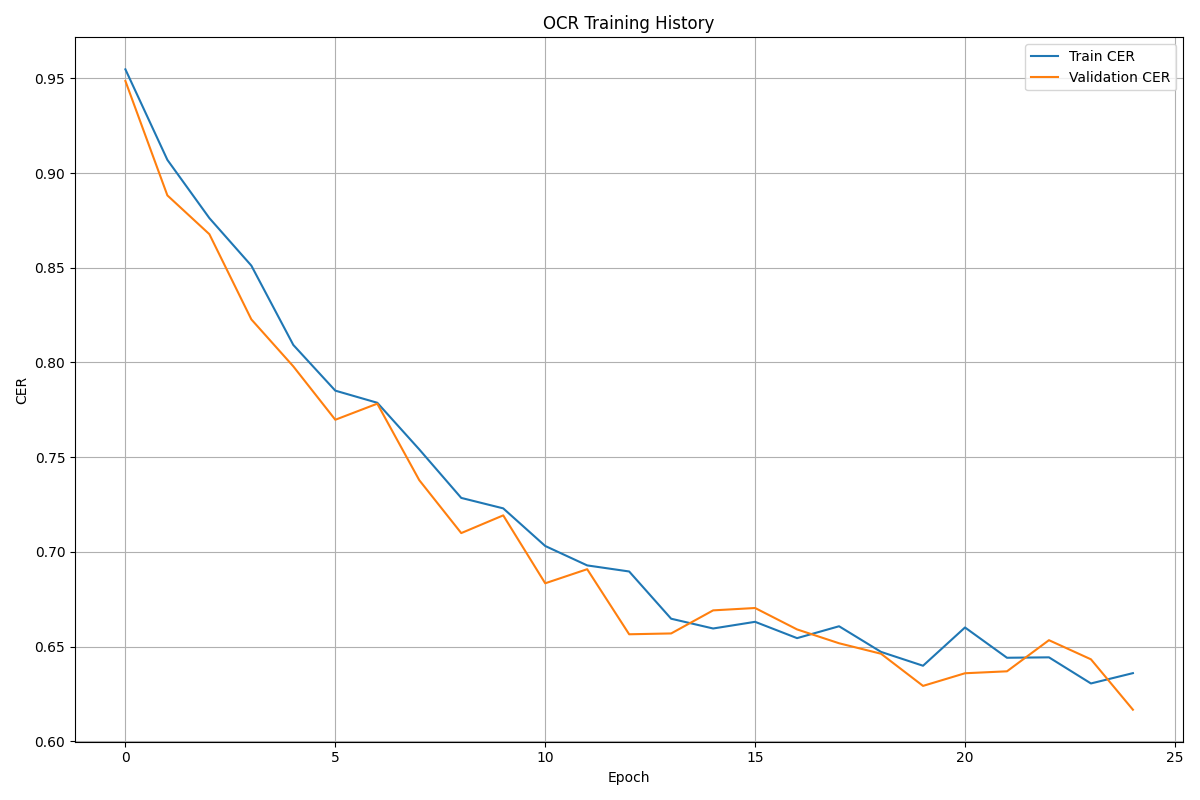
\includegraphics[width=\textwidth]{ocr_training_history} \caption{OCR modell tanítási és validációs karakterhiba-arány (CER) értékei} \label{fig-ocr-training} \end{figure}

A \emph{tesztelés} során kiderült, hogy a modell jelentős problémákkal küzd az \emph{ékezetes karakterek} felismerése terén. Különösen az ,,á'', ,,é'', ,,ő'' és ,,ű'' betűk okoztak nehézséget, amelyeket gyakran ékezet nélküli megfelelőikként azonosított. Emellett a \emph{szóközök felismerése} is következetlen volt, ami különösen a nevek feldolgozásánál okozott problémákat, mivel ezeket gyakran egybeírta vagy indokolatlanul több részre tagolta.

A \emph{határoló doboz detektáló modell} jóval meggyőzőbb eredményeket mutatott, amint az a \aref{fig-bbox-training} ábrán látható. A veszteségfüggvény értékei egyenletesen csökkentek, míg a pontosság már a korai epochokban is 90\% feletti értéket ért el, majd 98\% körül stabilizálódott.

\begin{figure} \centering 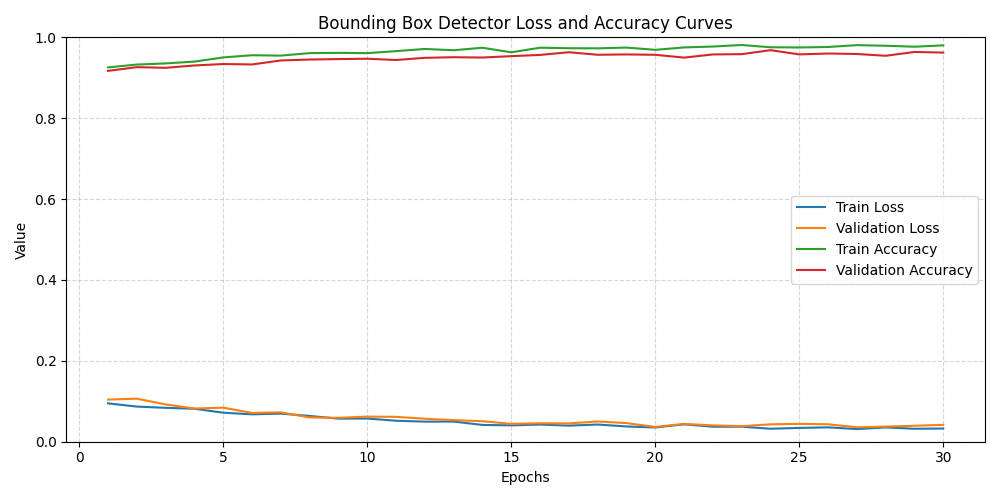
\includegraphics[width=\textwidth]{ideal_learning_curves} \caption{Határoló doboz modell tanítási folyamata - pontosság és veszteség} \label{fig-bbox-training} \end{figure}

Ugyanakkor a tesztelés során kiderült, hogy a modell érzékeny a \emph{perspektívatorzításra}. Amikor a felhasználók \emph{ferdén fotózták} a személyi igazolványt (20 foknál nagyobb szögben), a határdobozok jelentősen \emph{elcsúsztak}, ami az OCR modell számára tovább nehezítette a pontos szövegfelismerést. Különösen a kártya alsó részén található mezők (lejárati dátum, CAN kód) esetében volt észlelhető ez a probléma.

A \emph{nemfelismerő modell} teljesítménye a \aref{fig-gender-training} ábrán látható. A validációs pontosság csak lassan emelkedett, és a görbék mutatnak némi instabilitást. Az accuracy értéke a 40. epochra is csak 75\% körül stabilizálódott.

\begin{figure} \centering 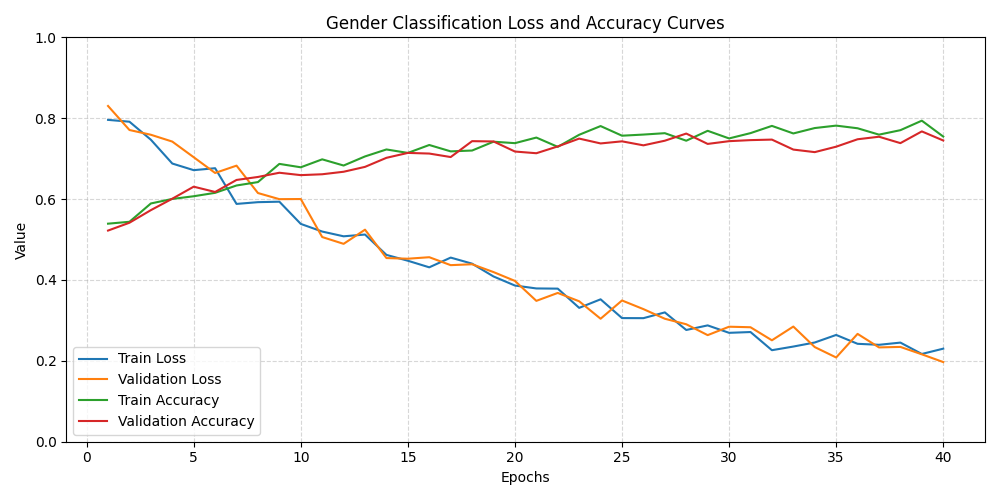
\includegraphics[width=\textwidth]{gender_learning_curves} \caption{Nemfelismerő modell tanítási és validációs metrikái} \label{fig-gender-training} \end{figure}

A nemfelismerő modell jelentős nehézségekkel küzdött bizonyos esetekben. A \emph{hosszú hajú férfiakat} gyakran nőként azonosította, míg a \emph{rövid hajú nőket} férfiként. Ez a jelenség rávilágít, hogy a modell túlságosan a kulturális sztereotípiákra (pl. hajhosszra) támaszkodik a nemek meghatározásánál, ahelyett hogy az arc más jellemzőit venné figyelembe. Idősebb személyek esetében is magasabb volt a téves osztályozás aránya.

\subsection{Eredmények kiértékelése} Az \emph{OCR modell} kezdeti tesztelésekor alacsony pontosságot ért el. A \emph{felismert karakterek} közel harmadában előfordult valamilyen \emph{hiba}, különösen az \emph{ékezetes betűk} esetében. A többszöri \emph{finomhangolás} után azonban sikerült a teljesítményt jelentősen javítani.

A \emph{határoló doboz detektáló modell} magas átlagos pontosságot ért el, ami összhangban van a tanulási görbén látható kiváló eredményekkel. A modell tanulási folyamata rendkívül stabil volt, már a korai szakaszban is magas teljesítményt mutatott. A perspektívatorzítás problémája azonban továbbra is fennáll, ami a valós használat során komoly korlátot jelenthet.

A \emph{nemfelismerő modell} kezdeti \emph{gyenge teljesítményét} jól tükrözi a tanulási görbe lassú emelkedése. Több javítási kísérlet után javult a pontosság, de még mindig elmarad az ideálistól. A modell túlzottan támaszkodik a felszíni jellemzőkre, mint a hajhossz vagy az arcforma, ami különösen problémás a nem szokványos megjelenésű személyek esetében.

A tanulási görbék elemzése alapján egyértelműen a \emph{határoló doboz detektáló modell} teljesített a legjobban, míg a nemfelismerő modell maradt a leggyengébb láncszem. Az OCR modellnél a CER értéke még a tanítás végén is viszonylag magas maradt, ami jelzi, hogy további fejlesztésekre lenne szükség.

A \emph{fejlesztési javaslatok} között szerepel az \emph{OCR modell} számára nagyobb és változatosabb, különösen ékezetes karaktereket tartalmazó adathalmaz használata, a \emph{nemfelismerő modellhez} komplexebb architektúra kidolgozása, amely kevésbé támaszkodik sztereotipikus megjelenési jellemzőkre, valamint a \emph{határoló doboz modellhez} automatikus perspektíva-korrekció beépítése, amely kompenzálja a ferdén készített fényképek torzítását.

Ezek a fejlesztések együttesen javíthatják a rendszer \emph{megbízhatóságát} és \emph{pontosságát} valós használati körülmények között, bár a jelenlegi állapotában is használható alapot nyújt a személyi igazolványok feldolgozásához, különösen emberi ellenőrzés mellett.
\end{document}